\section{Network Analysis}
\label{sec:network_analysis}

We analyze data on the network configuration of \acrshort{LDAP} instances and the \gls{TLS} configuration of \gls{LDAP} servers. We say an LDAP server's \gls{TLS} configuration is \enquote{without (potential) issues} when it fulfills two conditions: it has a valid X.509 chain, signed by a known root certificate of a \gls{CA} from a root store, and it follows the respective recommendations from RFC 9325 \cite{rfc9325} guidelines for connection security.

\iffalse
logic in the code:
cipher	   chain	result
----------------------------
rec	       valid	strong
rec	       invalid	weak
not rec	   valid	weak
not rec	   invalid	weak
\fi
\paragraph{Hosting.}

We use the IP2Location dataset to determine in which countries and networks \acrshort{LDAP} instances are deployed and summarize this in \cref{tab:results_overview}. More than 50\% of \acrshort{LDAP} servers are hosted in the US, Germany, France, Poland, Russia, or China. As shown in \cref{tab:ip_usage}, nearly half of the instances are located in networks that IP2location classifies as data centers, \ie a form of hosting. 
%Interestingly, more than 20\% and 14\% are allocated to network ranges classified as fixed-line or mobile ISPs. This classification \textit{may} indicate self-hosting situations. We note, however, that these categories are rather broad, with blurry boundaries, because ISPs often have many network ranges, for many different purposes, which also change over time.
Interestingly, 39.02\% are located in network ranges classified as \glspl{ISP}. This classification \textit{may} indicate self-hosting situations. We note, however, that these categories are rather broad, with blurry boundaries as \glspl{ISP} often have multiple network ranges for various purposes, which also change over time. 
Hence, we take this classification with a grain of salt. We also find a sizable number of \acrshort{LDAP} servers in commercial settings (7.32\%) or education (4.16\%). Outside the top four, we also find some deployment in government networks (0.40\%) or military networks (0.01\%). In all categories, we find servers associated with leaked passwords and personal data---including some in government or military networks.%\todo{RH: Once I have absolute numbers, or understand to which numbers the percentages in the table refer, I can add some text about leaks.}

% Surprisingly, we found Government and Military networks where it is possible to obtain passwords and personal information. We followed coordinated disclosure (see more at \cref{sec:ethics}).



%\cref{tab:ip_usage} highlights the usage of LDAP servers. Data centers, ISPs, companies, and educational facilities account for most LDAP servers openly at the Internet scale, which serves the purpose of many users and resources stored in an LDAP directory.

%\subsection{LDAP Churn Rate}

%\begin{figure}
%    \centering
%    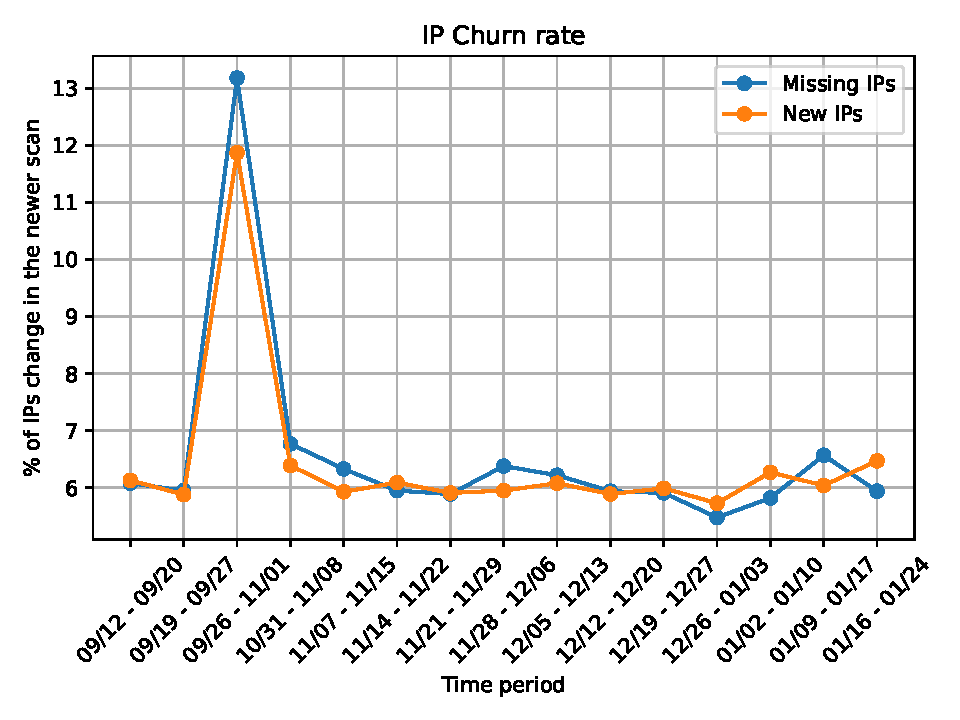
\includegraphics[width=0.47\textwidth]{img/ip_churn_rate.pdf}
%    \caption{LDAP IP Churn rate.}
%    \label{fig:ip_churn_rate}
%\end{figure}

\paragraph{TLS Cipher Suites.}
%\todo{The problem with ``static'' IPs again. What is our argument that we use the ``static'' hosts as a reference number? In reality, it is because we did not have FHM's IPs from their zmap scans early because those scans were still. But we could now filter for that to avoid this entire problem.}
% https://blog.ip2location.com/knowledge-base/what-is-usage-type/
\begin{table}[!tb]
\centering
    \small
    \setlength{\tabcolsep}{5pt}
    \begin{tabular}{@{} l r @{\hspace{5pt}}rr @{}}
    \toprule
    \thead{Network} & \multirow{2}{*}{\thead{Total IPs}} & \multicolumn{2}{c}{\thead{Leaks}} \\
    \cline{3-4} \thead{usage type}& & \multicolumn{1}{@{} l}{\thead{Credentials}} & \thead{Personal data} \\ 
    \midrule
    \midrule
    Total & 92,109 (100\%) & 1,817 (100\%) & 12,179 (100\%) \\
\arrayrulecolor{gray!90}
\midrule
\arrayrulecolor{black}
    %https://blog.ip2location.com/knowledge-base/what-is-usage-type/ There is no "Fixed Line"
    \begin{tabular}[c]{@{}c@{}}Data Center\end{tabular} & 48.17\% & 49.04\% & 39.63\%  \\
    % Merged ISP
    %Fixed Line ISP & 21.14\% & 11.50\% & 22.33\% \\
    %\begin{tabular}[c]{@{}c@{}}Fixed Line/\\Mobile ISP\end{tabular} & 15.86\% & 15.47\% & 17.31\% \\
    ISP & 39.02\% & 26.97\% & 41.18\% \\
    Commercial & 7.32\% & 14.91\% & 9.24\% \\
    Educational & 4.16\% & 6.60\% & 8.19\% \\
    %Mobile ISP & 2.02\% & 0.83\% & 1.54\% \\
    % Content Delivery Network & 0.55\% & 1.27\% & 0.81\% \\
    %Government & 0.40\% & 0.06\% & 0.61\% \\
    %Organization & 0.32\% & 0.17\% & 0.20\% \\
    %Search Engine Spider & 0.04\% & 0.11\% & 0.15\% \\
    %Library & 0.01\% & - & 0.01\% \\
    %Military & 0.01\% & 0.06\% & 0.01\% \\
    \bottomrule
    \end{tabular}
    \caption{Network types where LDAP servers are located.}
    % \rh{Dropped everything after the Top 5. Numbers are low, and the categories too generic or hard to understand. We can mention military in the text as an \textit{absolute} number. }
    % The dropped rows in this table do not reflect up-to-date numbers
    \label{tab:ip_usage}
\end{table}



%Total:  82,129
%TLS-enabled: 48198 or 56k???
Our Network Analysis Module aggregates all IPs that successfully negotiated a TLS connection with the TLS server certificate, forming a TLS-enabled subset of 48.2k servers (58\% of all identified LDAP servers).

%Our TLS analysis for cipher suites and X.509 certificate validation aggregate datasets and filter by hosts that negotiated and we retrieved their TLS certificates, forming a subset of the hosts expressed in \cref{tab:results_overview}.

%Only about 60\% (56k) of the candidate hosts respond to our scans with a successful \acrshort{TLS} connection. This is expected: recent findings by Sattler \etal~\cite{Sattler2023} and Izhikevich \etal~\cite{Izhikevich2022} show that many IPv4 addresses respond to a SYN packet but do not follow through with a full TCP handshake.

TLS defines several cipher suites, indicating the symmetric cipher, encryption mode, hash algorithm, and the key exchange method. We evaluate the established TLS connections against the best practices and recommended cipher suites from RFC 9325~\cite{rfc9325}.
As described in detail in \cref{appendix:tls}, only 65.92\% of the hosts use a recommended TLS cipher suite. This number decreases with servers that leak credentials (36.59\%), expose personal data (44.20\%), or expose internal information (61.42\%).

Servers that leak credentials use recommended cipher suites significantly less frequently (see \cref{tab:tls_overview} in \cref{appendix:tls}). The same is true for servers for which we find at least one CVE and, to a lesser degree, also for servers that contain personal data. Servers that provide support for \acrshort{SASL} or hold internally relevant, security-critical information, however, tend to fare better, but the situation is still not satisfactory. For example, around 40\% of these servers still use other cipher suites than recommended by the RFC. Overall, this paints a picture where weaker cryptography correlates with sensitive data leakages.


%A number of cipher suites are defined for use in \acrshort{TLS}. They indicate the symmetric cipher, block mode (if applicable), and the hash algorithm for the MAC. In addition, they indicate how the session key for the symmetric cipher was derived. In our evaluation, we generally refer to RFC 9325~\cite{rfc9325}, which defines best practices for \acrshort{TLS}. \todo{Gustavo: please add which conditions we do not check, if it is not too detailed}. In particular, the key exchange should always be ephemeral Diffie-Hellman (DHE) to enable forward security, ideally on elliptic curves. Classic finite-field Diffie-Hellman is discouraged for \acrshort{TLS} 1.2, and non-ephemeral Diffie-Hellman is generally viewed as too weak. Among the block modes in use, \acrlong{GCM} is considered secure, whereas CBC is (at least with Web protocols) under pressure due to padding oracle attacks~\cite{_PaddingOraclesDecline_2016} that are possible. Older hashing algorithms such as SHA1 are considered deprecated and should not be used anymore; the more modern SHA2 and SHA3 variants or the Poly1305 family of hash functions should be used instead. We refer to the RFC for details. \cref{tab:tls_overview} summarizes our findings.

%\todo{Explain that issue with the ``static'' hosts}. Most \acrshort{TLS} connections do not use the recommended cipher suites. We find RSA-based key exchange \todo{surprisingly often} (\todo{percentage across all TLS versions}). Other non-recommended cipher suits \todo{rely on CBC mode}.

%Following information are not shown in Table  \cref{tab:results_overview} ??
%However, a good number of connections (around 35\%) do use strong cipher suites. For example, across all \acrshort{TLS}-supporting \acrshort{LDAP} instances, we find that AES in Galois Counter Mode (GCM) is widely used (nearly 20\% of hosts), often even with a very secure key length of 256 bit. The modern stream cipher ChaCha20 makes for more than 16\% as well. These numbers change when we look at the percentages of servers that are insecure in some way. Servers that leak credentials commonly use strong cipher suites significantly less frequently. The same is true for server versions for which we find at least one CVE and, to a lesser degree, also for servers that contain personal data. Servers that provide support for \acrshort{SASL} or hold internally relevant, security-critical information, however, tend to be more commonly configured with better cryptography. Yet this is still unsatisfactory: for example, more than 50\% of servers that hold information of the latter kind still use non-recommended cipher suits. Overall, this paints a picture where weaker cryptography correlates with leakages of sensitive data.

%\begin{table*}[tb]
\centering
\small
\begin{tabular}{@{}lrrrrrr @{}}
\toprule
& \thead{Total IPs}     & \thead{Leak credentials} & \thead{Personal data} & \thead{SASL support}  & \thead{CVE}         & \thead{Internal info.} \\ 
\midrule
\midrule
Supporting TLS         & 48,198 (100\%) & 910 (100\%)      & 7,378 (100\%)  & 18,502 (100\%) & 528 (100\%) & 7,118 (100\%)   \\
\arrayrulecolor{gray!90}
\midrule
\arrayrulecolor{black}
Recommended            & 65.92\%       & 36.59\%          & 44.20\%       & 57.49\%       & 94.89\%     & 61.42\%        \\
Other       & 34.08\%       & 63.41\%          & 55.80\%       & 42.51\%       & 5.11\%      & 38.58\%        \\
... RSA (key exchange) & 24.27\%       & 57.14\%          & 53.71\%       & 41.77\%       & 5.11\%      & 36.93\%        \\
... CBC mode           & 12.26\%       & 8.35\%           & 6.3\%         & 3.64\%        & 5.11\%      & 5.49\%         \\
... 3DES               & 0.31\%        & 0.00\%           & 0.03\%        & 0.00\%        & 0.00\%      & 0.00\%        \\
\bottomrule
\end{tabular}
\caption{Recommended and non-recommended cipher suites on LDAP hosts supporting TLS.}
\label{tab:ciphersuites}
\end{table*}


%used in a TLS connection between client and server. The goal is to ensure communication confidentiality, data integrity, and server authenticity. Cipher suites tell, in a TLS session, the key exchange algorithms used to share the session secret key, the algorithm used to authenticate the server's identity, the encryption, and the hash algorithms used.

%We compare static LDAP servers with those where we found different categories of issues, as presented earlier.  Concerning non-recommended cipher suites, LDAP servers chose various forms of weak key exchange, authentication, encryption, and hash algorithms. For instance, key exchange using RSA is not recommended as it does not offer forward secrecy (\eg "TLS\_RSA\_WITH\_AES\_128\_GCM\_SHA256")~\cite{rfc9325}.

% When RSA is used to authenticate the server's identity (\eg "TLS\_ECDHE\_RSA\_WITH\_AES\_128\_GCM\_SHA256"), it is also recommended to use a certificate with at least 2048 bits of public key, which we see that a few servers do not follow. Encryption with AES in Cipher Block Chaining (CBC) stream cipher is also considered insecure (\eg "TLS\_RSA\_WITH\_AES\_128\_CBC\_SHA") as it is proven to be exploitable at the padding oracle attack~\cite{_PaddingOraclesDecline_2016}.

% Finally, SHA1 is considered insecure as collisions were~\cite{WangEtAlCollisionsSha1} found and have been declared deprecated since 2011 by NIST. 
% https://csrc.nist.gov/news/2022/nist-transitioning-away-from-sha-1-for-all-apps \cite{ComputerSecurityDivision_NISTTransitioningAway_2022}

\iffalse
\begin{figure}
    \centering
    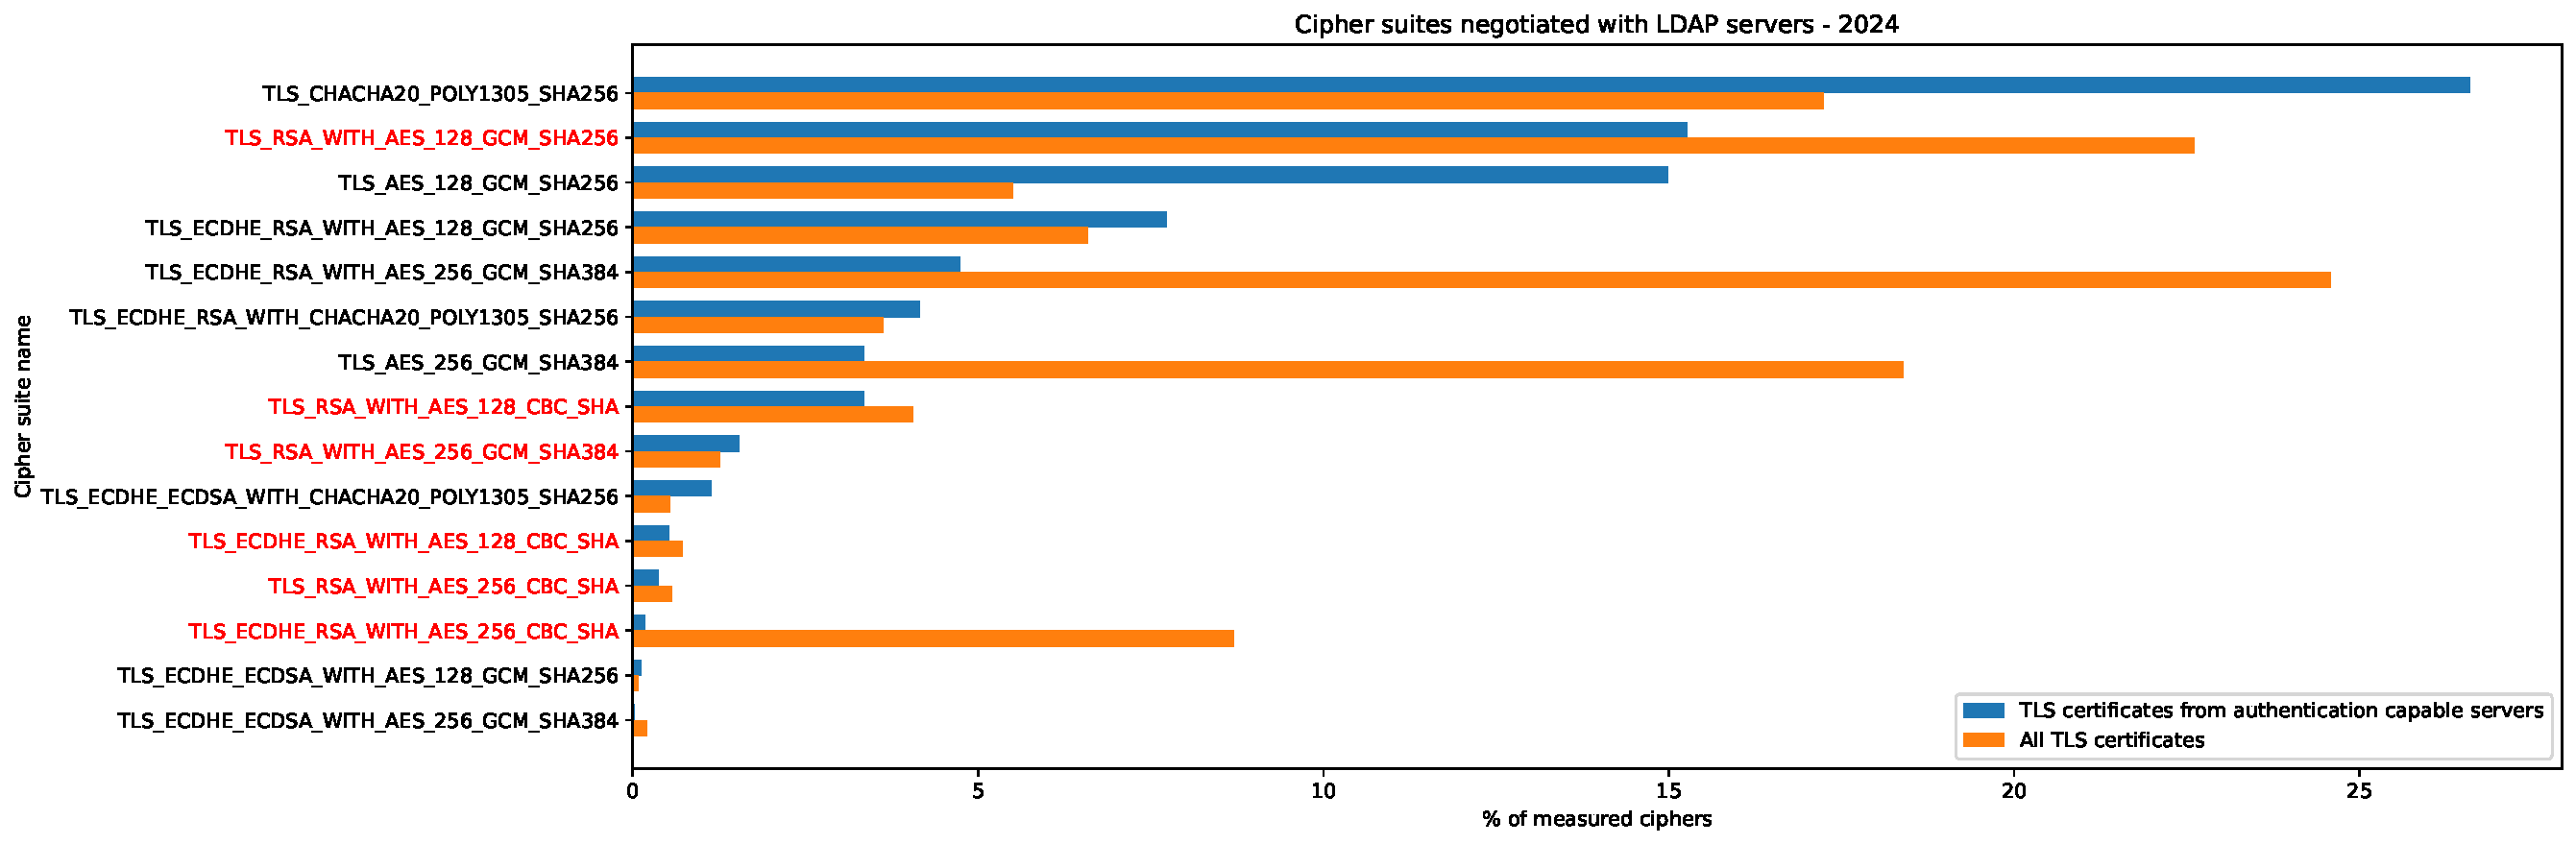
\includegraphics[width=0.47\textwidth]{img/cipher_suites.pdf}
    \caption{Cipher suites in TLS communication of LDAP servers.}
    \label{fig:cipher_suites}
\end{figure}
\paragraph{PII in plain text and weak TLS}
\paragraph{PII in plain with no implicit TLS and no STARTTLS}
\fi


%\begin{table*}[tb]
\centering
\small
\begin{tabular}{@{}lrrrrrr@{}}
\toprule
 & \thead{Total IPs} & \thead{Leak credentials} & \thead{Personal data}  & \thead{SASL support}   & \thead{CVE} & \thead{Internal info.} \\ 
\midrule
\midrule
Supporting TLS & 48,198 (100\%) & 910 (100\%) & 7,378 (100\%) & 18,502 (100\%) & 528 (100\%) & 7,118 (100\%) \\
\arrayrulecolor{gray!90}
\midrule
\arrayrulecolor{black}
TLSv1.3 & 36.67\% & 20.00\% & 27.24\% & 42.04\% & 28.41\% & 49.34\% \\
TLSv1.2 & 59.46\% & 77.03\% & 68.91\% & 55.92\% & 71.59\% & 46.90\% \\
TLSv1.1 & 0.33\%  & 0.33\%  & 0.16\%  & 0.23\%  & 0.00\%  & 0.10\% \\
TLSv1.0 & 3.54\%  & 2.64\%  & 3.69\%  & 1.81\%  & 0.00\%  & 3.67\% \\
\bottomrule
\end{tabular}
\caption{TLS version used in connections}
\label{tab:tls_version}
\end{table*}

\gls{TLS} 1.3 experienced a fast deployment on the Web, in part because of the widespread use of cloud hosting~\cite{Holz2020}. After just a few years, the deployment already exceeded 30\% on popular domains. For LDAP today, 36.67\% of all our identified TLS-enabled servers support TLS 1.3. Once again, the numbers are significantly lower for servers that leak sensitive information.


\paragraph{X.509 Chain Validation.}
%\begin{table*}[tb]
\small
\begin{tabular}{@{}lrrrrrr @{}}
\toprule
& \thead{Total IPs} & \thead{Leak credentials} & \thead{Personal data} & \thead{SASL support}  & \thead{CVE} & \thead{Internal info.} \\ 
\midrule
\midrule
Supporting TLS & 48,198 (100\%) & 910 (100\%) & 7,378 (100\%) & 18,502 (100\%) & 528 (100\%) & 7,118 (100\%) \\
\arrayrulecolor{gray!90}
\midrule
\arrayrulecolor{black}
Valid                     & 36.81\% & 17.69\% & 24.10\% & 40.38\% & 32.20\% & 47.78\% \\
Invalid                   & 63.19\% & 82.31\% & 75.9\% & 59.62\% & 67.80\% & 52.22\% \\
... Self-signed           & 32.30\% & 21.87\% & 22.61\% & 16.53\% & 1.70\% & 10.97\% \\
... Expired/not yet valid & 19.65\% & 43.63\% & 35.52\% & 25.15\% & 6.63\% & 14.34\% \\
... Unknown authority     & 11.20\% & 16.70\% & 17.74\% & 17.91\% & 59.28\% & 26.89\% \\
\bottomrule
\end{tabular}
\caption{X.509 certificate chain validation. Other errors rather than listed are less than 1\%.}
\label{tab:cert_chain}
\end{table*}

\iffalse
\begin{table}[tb]
\centering
\small
\begin{tabular}{@{}lrr@{}}
\toprule
\thead{Server type}& \thead{Supporting TLS} & \thead{Invalid X.509 chain} \\
\midrule
\midrule
Total         & 48,198 (100\%) & 63.19\% \\
\arrayrulecolor{gray!90}
\midrule
\arrayrulecolor{black}
Leak credentials  & 910 (100\%) & 82.31\% \\
Personal data     & 7378 (100\%) & 75.90\% \\
SASL support      & 18,502 (100\%) & 59.62\% \\
CVE               & 528 (100\%) & 67.80\% \\
Internal info.    & 7,118 (100\%) & 52.22\% \\
\bottomrule
\end{tabular}
\caption{X.509 certificate chain validation.}
\label{tab:cert_chain2}
\end{table}
\fi

%In this paper, we follow the Baseline Requirements for Certificate Authorities as currently established for the Web~\cite{_BaselineRequirementsTLS_}.

We find that over 50\% of the X.509 chains are \textit{globally invalid} as per our definition. The most common reasons for invalid chains are the use of self-signed certificates, expired or not yet valid certificates, and an unknown root certificate. For the latter case, we note the caveat of in-house CAs---we cannot detect these with our methodology, and hence this number needs to be treated as an upper bound. We note that self-signed certificates can be used in very bespoke situations to bypass the need for an in-house CA, \eg private servers used by one or very few clients. We summarize our results in \cref{tab:tls_overview}. We find very few cases where chains are invalid for other reasons (less than 1\%) (\eg self-signed certificates used to sign other certificates, too many intermediate certificates in the chain, violating path length constraints~\cite{rfc5280}, or improper use of critical extensions).

\begin{table}[tb]
\small
\setlength{\tabcolsep}{4pt}
\centering
\begin{tabular}{@{}lrrrrr@{}}
\toprule
 \thead{LDAP Client} & \thead{Total} & \thead{Rec.} & \thead{Other} & \thead{CBC mode} \\
\midrule
\midrule
Apache LDAP Studio & 38,269 & 71.82\% & 28.18\% & 11.97\% \\
LDAP Administrator & 38,545 & 69.98\% & 30.02\% & 13.15\% \\
ldapsearch         & 37,775 & 69.86\% & 30.14\% & 12.44\%  \\
Outlook            & 38,771 & 70.69\%  & 29.31\% & 12.27\% \\
Thunderbird        & 38,560 & 66.18\% & 33.82\% & 11.89\% \\
\bottomrule
\end{tabular}
\caption{Simulating the outcome of cipher suite negotiations using the cipher suites preferred by common LDAP clients.}
\label{tab:ClientHelloCipherSuites}
\end{table}


%\begin{table*}[!ht]
%\small
%\centering
%\begin{tabular}{@{}lrrrrr@{}}
%\toprule
% & \thead{Apache LDAP Studio} & \thead{LDAP Administrator} & \thead{ldapsearch} & \thead{Outlook} & \thead{Thunderbird} \\
%\midrule
%\midrule
%Supporting TLS & 38,269 (100\%) & 38,545 (100\%) & 37,775 (100\%) & 38,771 (100\%) & 38,560 (100\%) \\
%\midrule
%Recommended & 71.82\% & 69.98\% & 69.86\% & 70.69\% & 66.18\% \\
%Others & 28.18\% & 30.02\% & 30.14\% & 29.31\% & 33.82\% \\
%CBC mode & 11.97\% & 13.15\% & 12.44\% & 12.27\% & 11.89\% \\
%\bottomrule
%\end{tabular}
%\caption{Simulating the outcome of cipher suite negotiations using the cipher suites preferred by common LDAP clients.}
%\label{tab:ClientHelloCipherSuites}
%\end{table*}
\paragraph{Cipher Suites Chosen by LDAP Clients.} After our initial analyses, we also ran reconfirmation scans to understand how well our scanning methodology approximates the cipher suite negotiation that common LDAP clients would achieve.
We chose the five common LDAP implementations: Apache LDAP studio \cite{apacheldapstudio}, LDAP Administrator \cite{ldapadministrator}, \textit{ldapsearch} \cite{LdapsearchCommandLineTool}, Microsoft Outlook, and Thunderbird. 
%We have not tested JXplorer \cite{jxplorer} because it sends the same client-hello as Apache LDAP studio, as both are Java-based platforms
%Apache's implementation derives from Eclipse and Java. LDAP administrator is a licensed Software from a private company. Furthermore, \textit{ldapsearch} is based on the OpenLDAP open-source project. Outlook and Thunderbird are under Microsoft and Mozilla support, respectively, where the latter is also an open-source project.
We extract the cipher suite string they use in the handshake and use these in our scanner to determine which cipher suites LDAP servers would select.
On inspection, we found that our Go library does not support some cipher suites that the clients do, so we do not test them. However, these do not offer a more secure connection than our library offers.
%On inspection, we find that our Go library does not support some of the weaker cipher suites that these clients offer \textit{in addition} to the stronger ones, so we do not test for these.
%However, we found that none of the scanned servers chose one of these unimplemented cipher suites when presented with the emulated client hellos, which is in line with TLS servers generally choosing the strongest supported cipher suite. %These cipher suites are weaker than what our Go library supports.
However, servers should always choose recommended cipher suites, and we find that the servers do not reject our connection attempts due to a failure to negotiate a cipher suite. Therefore, clients should always be able to negotiate the same connection security our scanner can. Hence, we conclude that our method of simulating common LDAP clients is a good approximation.

%use ephemeral DH, Elliptic Curve (EC) DH and ECDHE, \gls{CBC} mode for encryption, or RSA for key exchange. For compatibility reasons, the clients, except for Thunderbird and LDAP administrator, also offer TLS\_EMPTY\_RENEGOTIATION\_INFO\_SCSV. In summary, none of these cipher suites improved the connection security when connected to LDAP servers other than what our scanner already offers.

We summarize the results of these tests in \cref{tab:ClientHelloCipherSuites}, reusing our categorization of recommended ciphers. A more detailed description of the results is presented in \cref{appendix:tls}. We find that the numbers are within a small margin of our previous scans, and in general, the percentage of recommended cipher suites negotiated is actually slightly higher. As these reconfirmation scans took place five months after the original scans, this could simply be due to servers that have received updates meanwhile rather than any difference in the cipher suite negotiation. Our conclusion is that our scanning methodology approximates the behavior of real LDAP clients very well.



% RH: this here is possibly true pending a new check: how many root CAs have been rejected because of SHA1?
% We further investigated \iffalse(see \cref{fig:reasons_invalid_chains})\fi, and most are signed by unknown authorities, indicating self-signed certificates. 
%Another typical case of invalid chains is expired or not yet valid certificates.  The latter could be attributed to our client not being able to process such extensions or that it is broken. \cref{tab:proper_tls} summarizes the errors as invalid chains. We attribute the results to careless administration of the PKI of the LDAP ecosystem, which puts clients at risk while connecting to such LDAP servers.

%The TLS certificate validity window is the difference between the fields "not after" and "not before" from all hosts found stable in our scans, \ie not churning from one measurement to another. \cref{fig:certs_validity_window} shows that a set of TLS certificate expiration dates is carelessly set to arbitrary values, which at first let system administrators have the false perspective of a protected server, however long-life certificates, if not revoked, will be broken in the future.

\iffalse
\begin{figure}
    \centering
    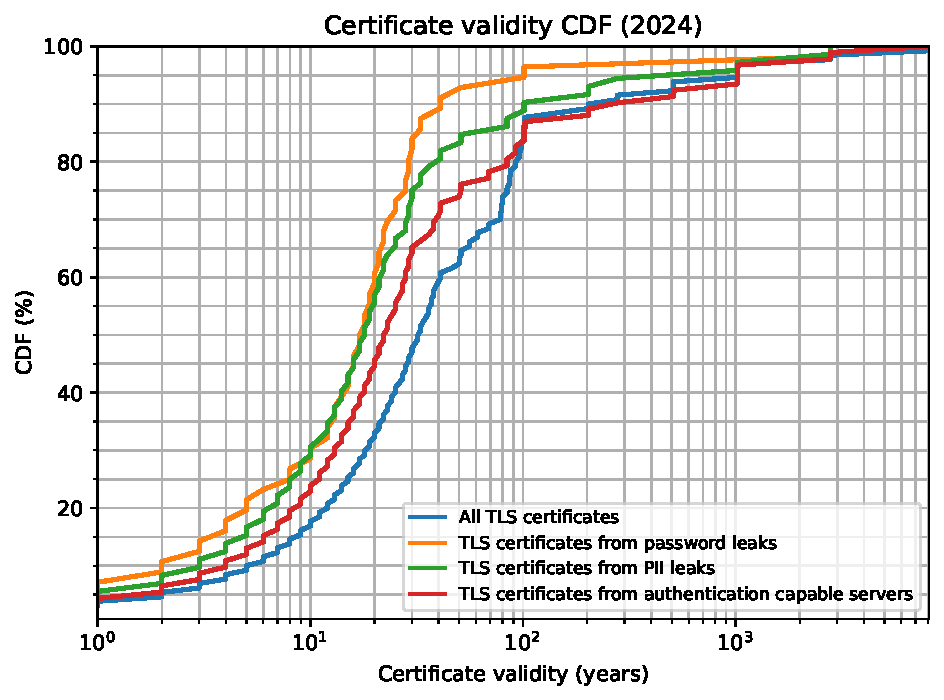
\includegraphics[width=0.45\textwidth]{img/validity_cdf_line.pdf}
    \caption{CDF of TLS certificates validity window}
    \label{fig:certs_validity_window}
\end{figure}
\fi


% Moved to Discussion!
%\paragraph{Summarizing view}
%\todo{Cross-check against tables!!! This was written before the final tables were in.}

%\begin{table*}[tb]
\centering
\small
\begin{tabular}{@{}lrrrrrr@{}}
\toprule
 & \thead{Total IPs} & \thead{Leak credentials} & \thead{Personal data}  & \thead{SASL support}   & \thead{CVE}          & \thead{Internal info.} \\ 
\midrule
\midrule
Supporting TLS & 48,198 (100\%) & 910 (100\%) & 7,378 (100\%) & 18,502 (100\%)  & 528 (100\%)  & 7,118 (100\%) \\
\arrayrulecolor{gray!90}
\midrule
\arrayrulecolor{black}
Strong TLS              & 14,920 (30.96\%) & 122 (13.41\%) & 1,392 (18.87\%) & 5,799 (31.34\%) & 157 (29.73\%) & 2,341 (32.89\%) \\
Weak TLS config         & 33,278 (69.04\%) & 788 (86.59\%) & 5,986 (81.13\%) & 12,703 (68.66\%) & 371 (70.27\%) & 4,777 (67.11\%) \\
... \begin{tabular}[c]{@{}l@{}}Not recommended\\ cipher suites\end{tabular} & 16,424 (34.08\%) & 577 (63.41\%) & 4,117 (55.80\%) & 7,866 (42.51\%) & 27 (5.11\%) & 2,746 (38.58\%) \\
... Invalid X.509 chain & 30,454 (63.19\%) & 749 (82.31\%) & 5,600 (75.90\%) & 11,030 (59.62\%) & 358 (67.80\%) & 3,717 (52.22\%) \\
\bottomrule
\end{tabular}
\caption{Overview of TLS connections and certificates.}
\label{tab:proper_tls}
\end{table*}
%\cref{tab:proper_tls} gives an overview of what we consider strong and weak \acrshort{TLS} configurations, breaking the reasons for weak configurations down into issues with the cipher suites vs. certificate chains. We see the already-established pattern again. Overall, just about a quarter of \acrshort{TLS} connections can be said to have a strong configuration. The number drops substantially in the case of servers that leak credentials (a mere 10\%) or personal data (about 13\%). It increases when servers are used for authentication or hold sensitive internal information. Servers that leak credentials or store personal data have particularly often poor configurations, both in terms of cipher suites and certificates. The strong correlation we see between weak cryptography and older \acrshort{TLS} version on the one hand, and data leakages and vulnerable \acrshort{LDAP} versions on the other hand, would support the hypothesis that the more weakly configured servers have not been updated in a number of years.